\documentclass[../main.tex]{subfiles}
%!TEX root = ./chapter1Introduction.tex
\graphicspath {{../}}

\begin{document}
\chapter{Introduction}
%---------------------------------------------------------------------
%	PROJECT MANDATE
%---------------------------------------------------------------------
\section{Project Mandate} \label{Mandate}
The goal of the project is to overcome the current limitations involved with the control of unmanned airships in adverse outdoor conditions. The airship consists of a helium filled envelope, external keel, and gondola which will act as a ballast. The moving ballast will control the pitch by the controlled displacement of the centre of mass. Propulsion will be provided by propellers in the X-Y plane of the airship. The system will have vector thrusting to allow for altitude change independent of pitch change.

%---------------------------------------------------------------------
%	PROJECT SCOPE
%---------------------------------------------------------------------
\section{Group Problem Scope} \label{Scope}
The research project led by Dr. Eric Lanteigne involves designing a system to allow for the control of an unmanned airship. The goal of the project is to create a system that controls the airship by changing the position of the centre of mass to initiate pitch change. This pitch change, along with forward propulsion, will drive the airship in a given direction. The design team will be responsible for creating a system, where a gondola that acts as a ballast will move along a non-linear, diamond-shaped keel in order to initiate pitch change of an airship. Ideally, the system will be able to achieve a pitch change of up to ninety degrees, allowing the airship to descend straight downwards. Currently, all designs must be scalable as specifications of the airship envelope have yet to be finalized. The unmanned airship must be capable of flying outdoors in wet conditions and be able to carry a payload of between 0.2kg and 0.5kg. Landing/mooring will not be an issue, and thus is outside of the project scope, as it will be grabbed by an individual during descent.

%---------------------------------------------------------------------
%	CRITERIA AND RESTRICTIONS
%---------------------------------------------------------------------
\section{Criteria and Restrictions}
The propellers will be in the X-Y plane, in line with the centre of volume. This eliminates any moments from the propellers that lead to imbalance and unwanted pitch variations. The gondola will be able to move along the varying curvature of the keel using a hinged-gondola. The driving mechanism will be two friction wheels with the additional support of 4 driven bearings. The cross-section of the keel is diamond-shaped, however it is not torsionally constant due to imperfections in the manufacturing process. This means the vertexes are not coincident on the curved section. Once the airship has been constructed, a Special Flight Operations Certificate (SFOC) issued by Transport Canada will be necessary in order to fly the airship lawfully.

%---------------------------------------------------------------------
%	PARAMETERIZATION OUTLINE
%---------------------------------------------------------------------
\section{Parametrization Overview}
A high level overview of the system's parametrization is shown in Figure \ref{fig:ModellingOutline}.

\begin{figure}[H]
	\centering
	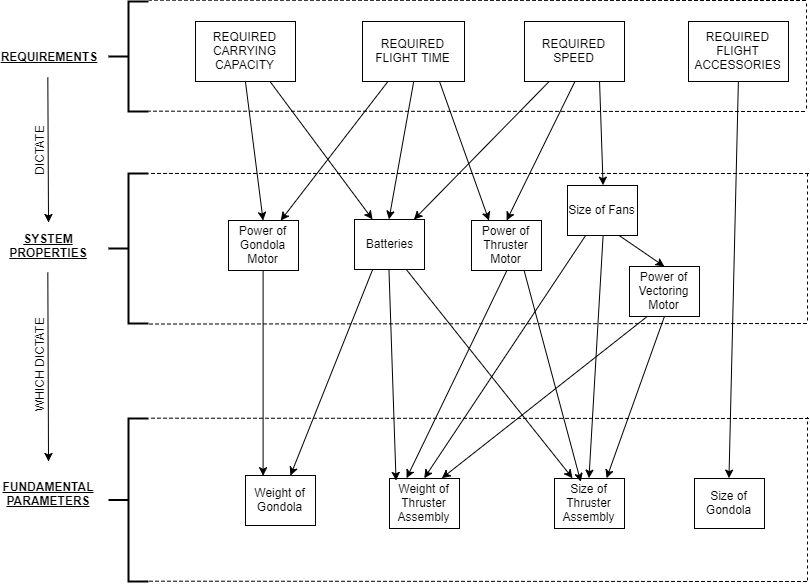
\includegraphics[width=\textwidth]{img/paramaterization/Brief_Overview.png}
	\caption{Overview of Modelling Parametrization}
	\label{fig:ModellingOutline}
\end{figure}

This outline conveys the extreme interdependencies involved in parametrizing the airship. Each input parameter impacts almost every output parameter, making total parametrization non-linear. The parametrization outline for the entire airship can be seen in Figure ??.

\end{document}